\documentclass[border=2pt]{standalone}
\usepackage{tikz}
\usetikzlibrary{trees}
\begin{document}
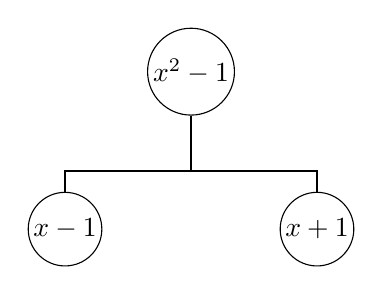
\begin{tikzpicture}[
  grow=down,
  level distance=20mm,
  sibling distance=32mm,
  every node/.style={draw,circle,minimum size=9mm,inner sep=1pt},
  edge from parent/.style={draw,thick},
  edge from parent path={
    (\tikzparentnode.south) -- +(0,-.35\tikzleveldistance) -| (\tikzchildnode.north)
  }
]
  \node {$x^2-1$}
    child {node {$x-1$}}
    child {node {$x+1$}};
\end{tikzpicture}
\end{document}
